\chapter{Evaluation}
\label{chap:evaluation}

\section{Testing}

When developing an algorithm library for formal analysis of safety
critical systems it is vital to verify the correctness of the
implementation. Since the complexity of the code base makes formal
verification difficult we confined ourselves to rigorously testing the
functionalities provided by the library.

In this section, we summarise work presented in%
~\citep{TDK2015_Klenik_Marussy} that was performed to verify the
correctness of our implementation of the data structure, operations
framework and the stochastic analysis algorithms.

\subsection{Combinatorial testing}

As described in \cref{chap:operations} algorithms use the common
vector and matrix data structure to perform various operations. This
makes the used storage techniques transparent which in turn makes the
code base more concise, reusable and less prone to errors.

The most important requirement concerning the data structure and
operations is mathematical correctness regardless of the storage
technique and manner of execution (e.g.~parallel or sequential)
used. Considering the number of implementations for a given interface
and the previous requirement we used a simple unit testing design
pattern (also known as interface testing pattern) as the core building
block for the data structure testing \citep{myers2011art}.

The basic idea behind this pattern is to write unit tests for
interface operations without any knowledge about the concrete
implementation. Hiding implemetation details can be achieved in a
number of ways. Some unit testing frameworks, such as \textsc{NUnit}%
~\citep{NUnit}, support the usage of generic test classes and running
them for multiple concrete types.

Since most of the time multiple instances of different types of
interface implementations are needed in a single unit test we choose a
more flexible approach for hiding implementation details. This
approach is based on class inheritance and abstract factory
methods. Whenever an instance if a given interface is needed, the
instantiation is delegated to an abstract factory method in the test
class.

\emph{Abstract test cases} were created to describe desired behaviors
of the operations. \emph{Concrete test cases} are derived from
abstract tests and contain calls to the data structure factory
methods. Thus, the behavior of any operatio may be tested for all
possible data structure calsses.

\subsubsection{Abstract tests}

Writing unit tests for valid parameter values is straighforward since
it is possible to cover multiple valid parameter ranges with a single
unit test. However testing for invalid parameter values requires some
care. There must only one invalid parameter per unit test lest one
error can obscure the others. This significantly increases the number
of unit tests. Therefore we aimed to gather every possible invalid
parameter range automatically.

We used Microsoft IntelliTest%
\footnote{formerly known as \textsc{Pex}~\citep{tillmann2008pex}}%
~\citep{IntelliTest}, which assists in automating white-box and unit
testing. IntelliTest automatically generates unit tests using
constraint satisfaction problem solving based on the source code of
the method under test. Using IntelliTest on our interface code
contract classes provided mmany invalid parameter values which were
used in abstact unit tests.

\subsubsection{Concrete tests}

Derived classes of abstract tests are created for every possible
combinations of data structure classes by implementing the abstract
factory method. Since the number of possible combinations is too large
to implement manually derived classes were generated with a Microsoft
Text Template Transformation Toolkit~(\textls{T4})~\citep{T4}
template.

Pairwise testing was used to decrease the number of generated tests
compared to full combinatorial testing of implementation
combinations. To generate the combinations for pairwise testing we
used the \textls{ACTS} tool \citep{borazjany2012combinatorial}.

As a result of this testing process more than $78\;000$ unit tests
were generated using full combinatorial testing (more than $18\;000$
with pairwise testing) which together with the behavior configuration
files serve as a quasi-formal specification for the expected behavior
of future and modified implementations (e.g.~perfomance
optimization).

Breaking changes in implementation should either be rejected or the
test suite and configuration files should be revised as specification
change. Every unit test was executed sucessfully for both sequential
and parallel operation implementations.

Concrete tests were executed with both configurations provided by the
operation framework as defaults, i.e.~parallel and sequential, to
ensure that computations are logically equivalent.

\subsection{Software redundancy based testing}

Apart from testing the datastructure operation implementations it is
vital to test the correctness of higher level algorithms used in the
analysis workflow, e.g.\ the linear equation solver and transient
analysis algorithms.

Testing every implemented algorithm with unit tests would be
tremendous work that cannot be easily automated or maintained.
Moreover, every algorithm is used as part of a bigger workflow which
raises the question of compatibility of algorithms during an analysis.

As described in \cref{chap:overview:sec:our-workflow} for almost every
step of the workflow numerous algorithms are available.

\begin{obs}
  \label{obs:evaluation:reward-results}
  The result of a performance analysis (e.g.\ reward calculation) is
  mathematically independent of the used analysis workflow. It only
  depends on the possible behaviors of the system and the definition
  of the required performance measure. Two results calculated by two
  different analysis methods can only differ from eachother due to the
  numercial precision properties of the algorithms.
\end{obs}  

Combining our fully configurable workflow with
\cref{obs:evaluation:reward-results} presents a new approach for
testing the algorithm implementations in a maintainable and almost
automatic manner. We can take advantage of the concept of software
redundancy commonly used in safety critical applications.

The main idea behind software redundancy is to perform a calculation
multiple times with usually fundamentally different algorithms
--~often developed by independent teams~-- thus minimizing the
possibility of common mode failures. After the calculations a voting
component examines whether every algorithm calculated the same
result. If that's not the case then one or more of the algorithms are
incorrect.

In this testing testing phaseg our analysis workflow is ran with a
given configuration and the calculated reward and sensitivity values
are saved. $588$ mathematically consistent configurations were
generated and executed on multiple benchmark models and case
studies. Tthe maximum absolute difference of the calculated results
was examined as an error indicator.

\section{Measurements}

In this section we introduce the models used throughout the testing
and benchmarking phase and present results about the performance of
solver algorithms using the sparse matrix and block Kronecker
decomposition matrix forms.

Every model used for testing and measurement is publicly available at
\url{https://github.com/kris7t/stochastic-analysis} in a variety of
stochastic modelling formats.

\subsection{Models}

\subsubsection{Shared resource}

\begin{figure}
  \centering
  \begin{tikzpicture}
    \runningExamplePetriNet
  \end{tikzpicture}
  \caption{Stochastic Petri net for the \emph{SharedResource}
    model.}
  \label{fig:evaluation:model:sharedresource}
\end{figure}

Benchmark models were generated based on the Stochastic Petri Net
(\textls{SPN}) \emph{SharedResource} model shown in
\cref{fig:evaluation:model:sharedresource}.

The model contains a number of clients competing for a central
resource ($p_S$). Each client may run a number of processes, which are
represented by token on $p_{C_i}$.

The model can be scaled by increasing the number of available shared
resources, the number of clients and the number of processes per
client. In \cref{ssec:evaulations:results}, $5$ clients were used and
the number of processes and shared resources were set to equal
values. In \cref{sec:evaulations:idrstab}, all parameters were sweeped
independently.

Symmetric, slightly asymmetric and significantly asymmetric versions
of the model were created by assigning transition rates. In the first
case, all transition rates are equal to $1$, while in the third case
there are orders of magnitude of difference between the transitions
rates.

\subsubsection{Kanban}

The \textls{SPN} model of \emph{Kanban} (\textls{KB}) manufacturing
process \citep{ciardo2003logical} was used as another benchmark
model. The model was scaled by modifying the available resources at
each stage of the model resulting in an increase in the size of the
state space.

\subsubsection{Cloud performability}

The represents a cloud architecture \citep{ghosh2012scalable} with
physichal and virtual machines serving incoming jobs using warm and
cold spare resources in case of increasing load. Some aspects of the
model in \citep{ghosh2012scalable} were modified because our library
currently does not support the Generalized Stochastic Petri Net
(\textls{GPSN}) formalism.

\subsection{Results}
\label{ssec:evaulations:results}

\section{The convergence of \textls[30]{IDRSTAB}}
\label{sec:evaulations:idrstab}

\begin{figurepage}
  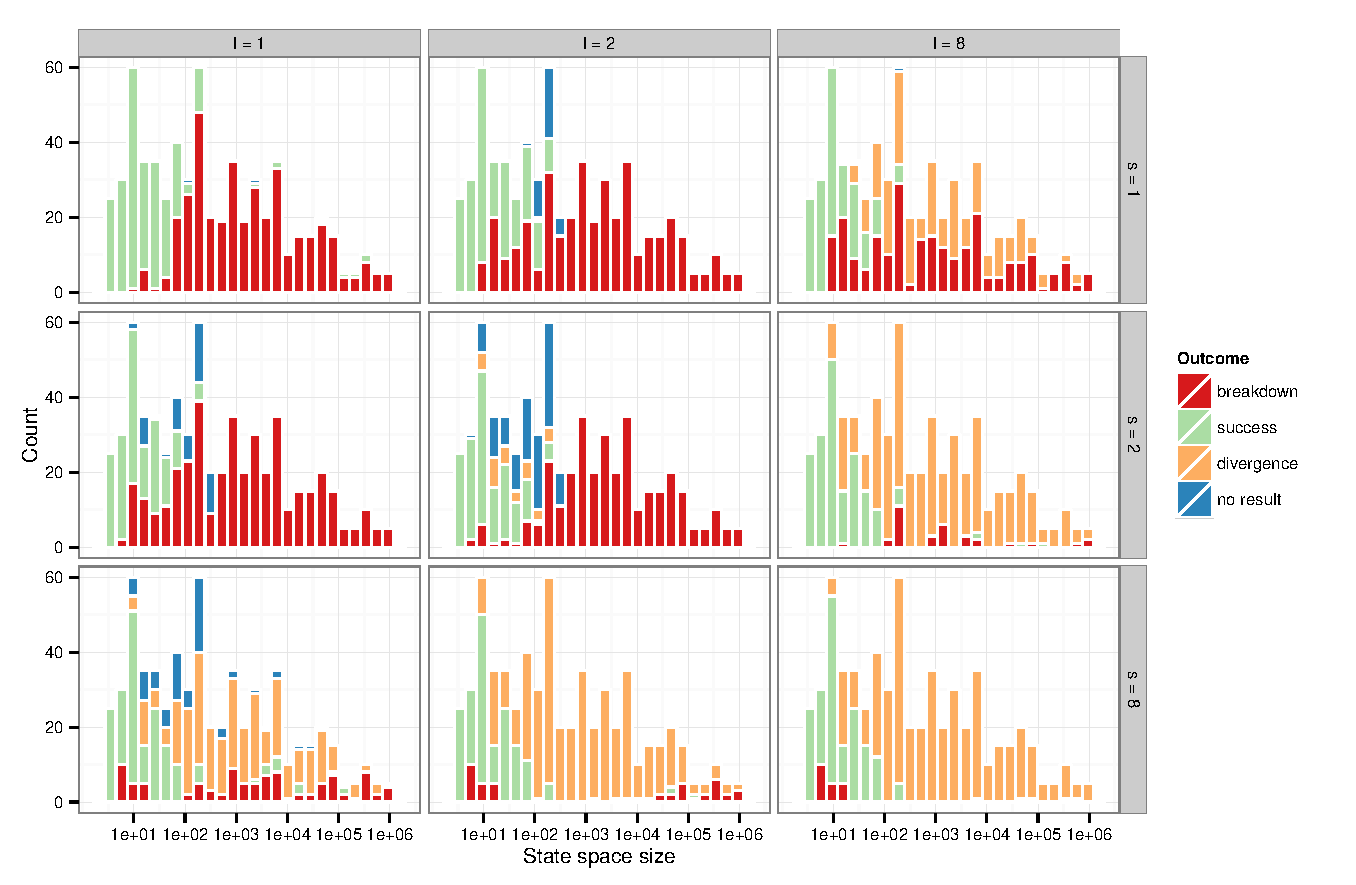
\includegraphics{figures/idrstab_histograms}
  \captionof{figure}{Histogram of observed behaviors of
    \textls{IDR}($s$)\textls{STAB}($\ell$).}
\end{figurepage}

\begin{figurepage}
  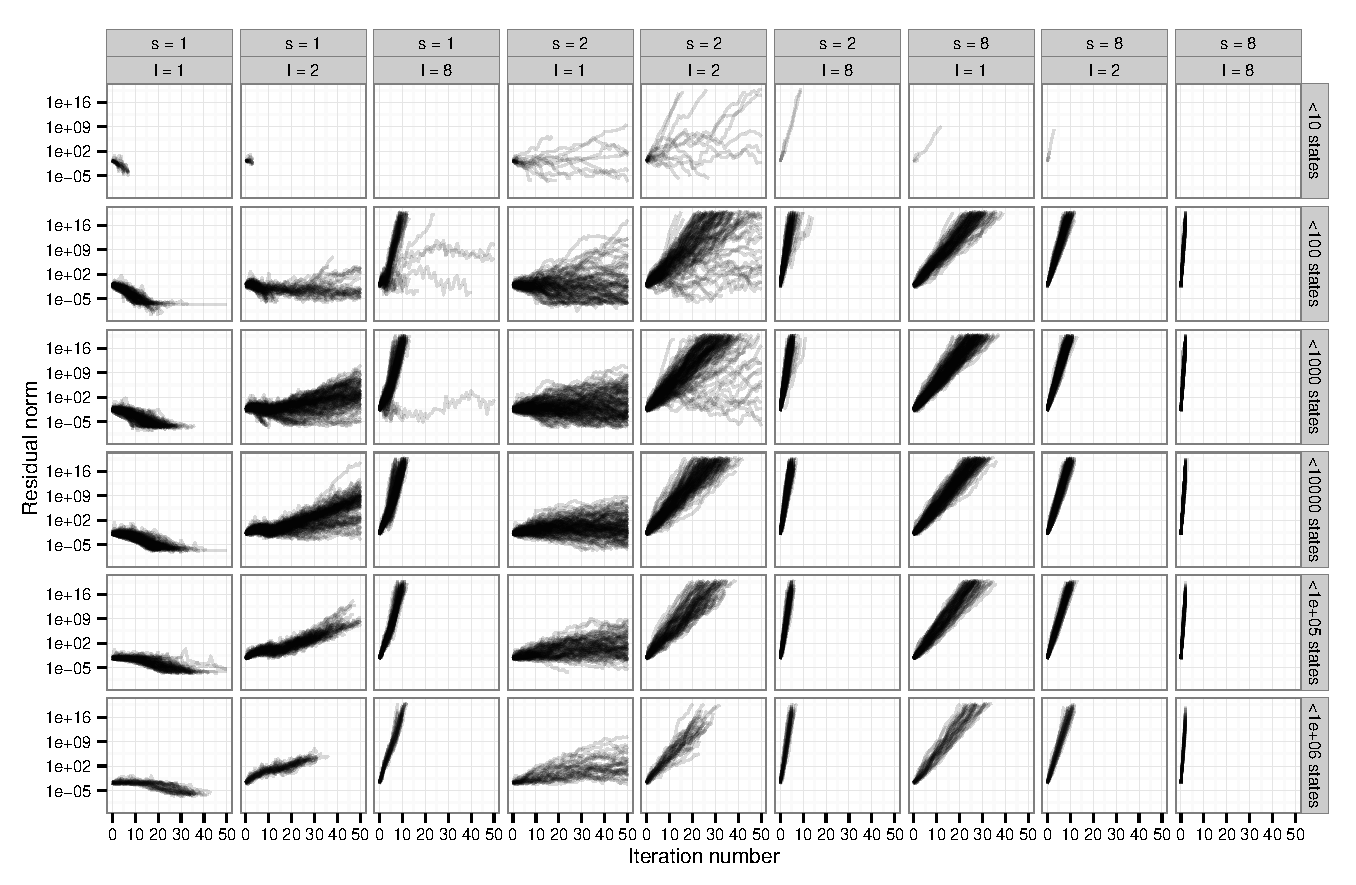
\includegraphics{figures/idrstab_convergence}
  \captionof{figure}{Convergence histories observed in various runs of
    \textls{IDR}($s$)\textls{STAB}($\ell$).}
\end{figurepage}
